\section{2. Alignment, sequence search, and primer design}

\begin{framed}
\textbf{Learning outcomes}\\
In this chapter, you will study sequence alignment.

Make sure you understand what DNA and protein alignments are used for and that you can explain the differences between local and global alignments.
You should be familiar with concepts related to alignments and sequence search, like dotplots, alignment scores, e-values, and substitution matrices.
Make sure you understand what multiple alignments are used for and that you can explain the differences between different solutions for the MSA problem.
You should understand what motifs are and the basics of profile hidden Markov models.
This chapter concludes with a section on PCR primer design as an example on the use of sequence alignment algorithms in practice.

During the practical you will learn how to make pairwise and multiple-sequence alignments, perform sequence searches and motif analyses, design primers, and discuss the results.
\end{framed}

\subsection{Introduction}

% #%[TODO: There can be more biological examples in this section]

Comparing DNA and protein sequences is a key tool in the field of applied bioinformatics.
By analyzing these sequences, researchers can annotate genes from new genomes, build models of protein structures, and investigate gene expression, i.e., which genes are turned on and off.
It is important to notice that nature tends to stick with what works, rather than reinventing the wheel for each species.
Instead, organisms evolve from ancestors, they accumulate mutations (Chapter~1), and gradually develop new traits over time.
That means that similar genes can be found in different organisms and the functional information can be transferred from one protein to another if both possess a certain degree of similarity.
However, even though two proteins may look similar, they could also have different functions.
Generally, similarities arise because of shared ancestry (divergent evolution), nevertheless, similarities can also appear independently (convergent evolution).

Before diving into the analysis of whether sequences are related, it is important to understand some key terms.

\begin{framed}
\textbf{Homology and similarity}\\
\textbf{Homology} means that sequences share a common evolutionary history and therefore have a common ancestor.
Homology is not quantifiable.
If two sequences have a common ancestor, they are homologous.
Thus, two sequences are either homologous or they are not.

\textbf{Sequence identity} and \textbf{sequence similarity} are often used to infer whether two sequences are homologous.
We can measure the identity or similarity between sequences and we will see how to do this later in this chapter.

In contrast, we cannot measure homology, but we can only infer it.
\end{framed}

\begin{framed}
\textbf{See also}\\
Here is a classic paper on homologous protein families: \href{https://pubmed.ncbi.nlm.nih.gov/9381173/}{Tatusov et al., 1997}.
\end{framed}

\subsection{Dot plots}

Dot plots are a simple way to visualize similar regions between two sequences.
They are represented by a two-dimensional array, where one sequence is written vertically and the other horizontally.
A dot is placed in a cell, where the residues are identical.
In the resulting plot, similar regions appear as diagonal stretches and insertions and deletions appear as a discontinuity in a diagonal line (Figure~\ref{dotsmall}).

\begin{figure}[!htbp]
\centering
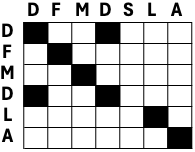
\includegraphics[width=0.9\linewidth]{files/dot_small2-db4f4d0b90fecfbd44f5897dc049fa70.png}
\caption[]{A small example of a dotplot. \newline
Credits: \href{https://creativecommons.org/licenses/by-nc/4.0/}{CC BY-NC 4.0} \cite{own_2_2024}.}
\label{dotsmall}
\end{figure}

A sequence can also be compared to itself, then the main diagonal will be filled with dots and additional repeats are on the off-diagonal (Figure~\ref{dotlarge}).

\begin{figure}[!htbp]
\centering
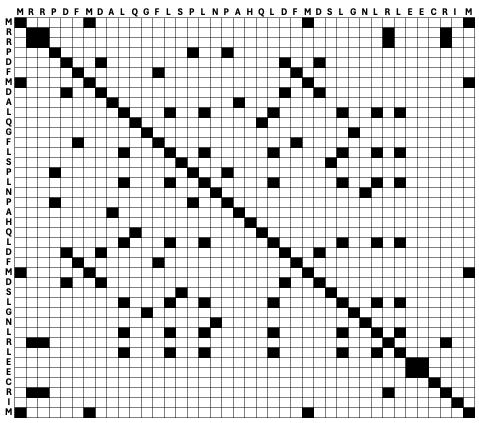
\includegraphics[width=1\linewidth]{files/dot_large-dc5236a779ddd7ca60530ad37c9d5291.png}
\caption[]{An example of a dotplot to compare a sequence with itself. Credits: \href{https://creativecommons.org/licenses/by-nc/4.0/}{CC BY-NC 4.0} \cite{own_2_2024}.}
\label{dotlarge}
\end{figure}

This simple way of marking identical residues shows a lot of background noise.
To detect interesting patterns, typically a filter is applied.
For example, a minimum identity should be present across a certain window size, i.e., consecutive number of residues being considered.
This feature is implemented in a webserver to visualize dotplots, \href{https://dotlet.vital-it.ch/}{dotlet} \cite{dotlet_2000} (Figure~\ref{dotweb}).

\begin{figure}[!htbp]
\centering
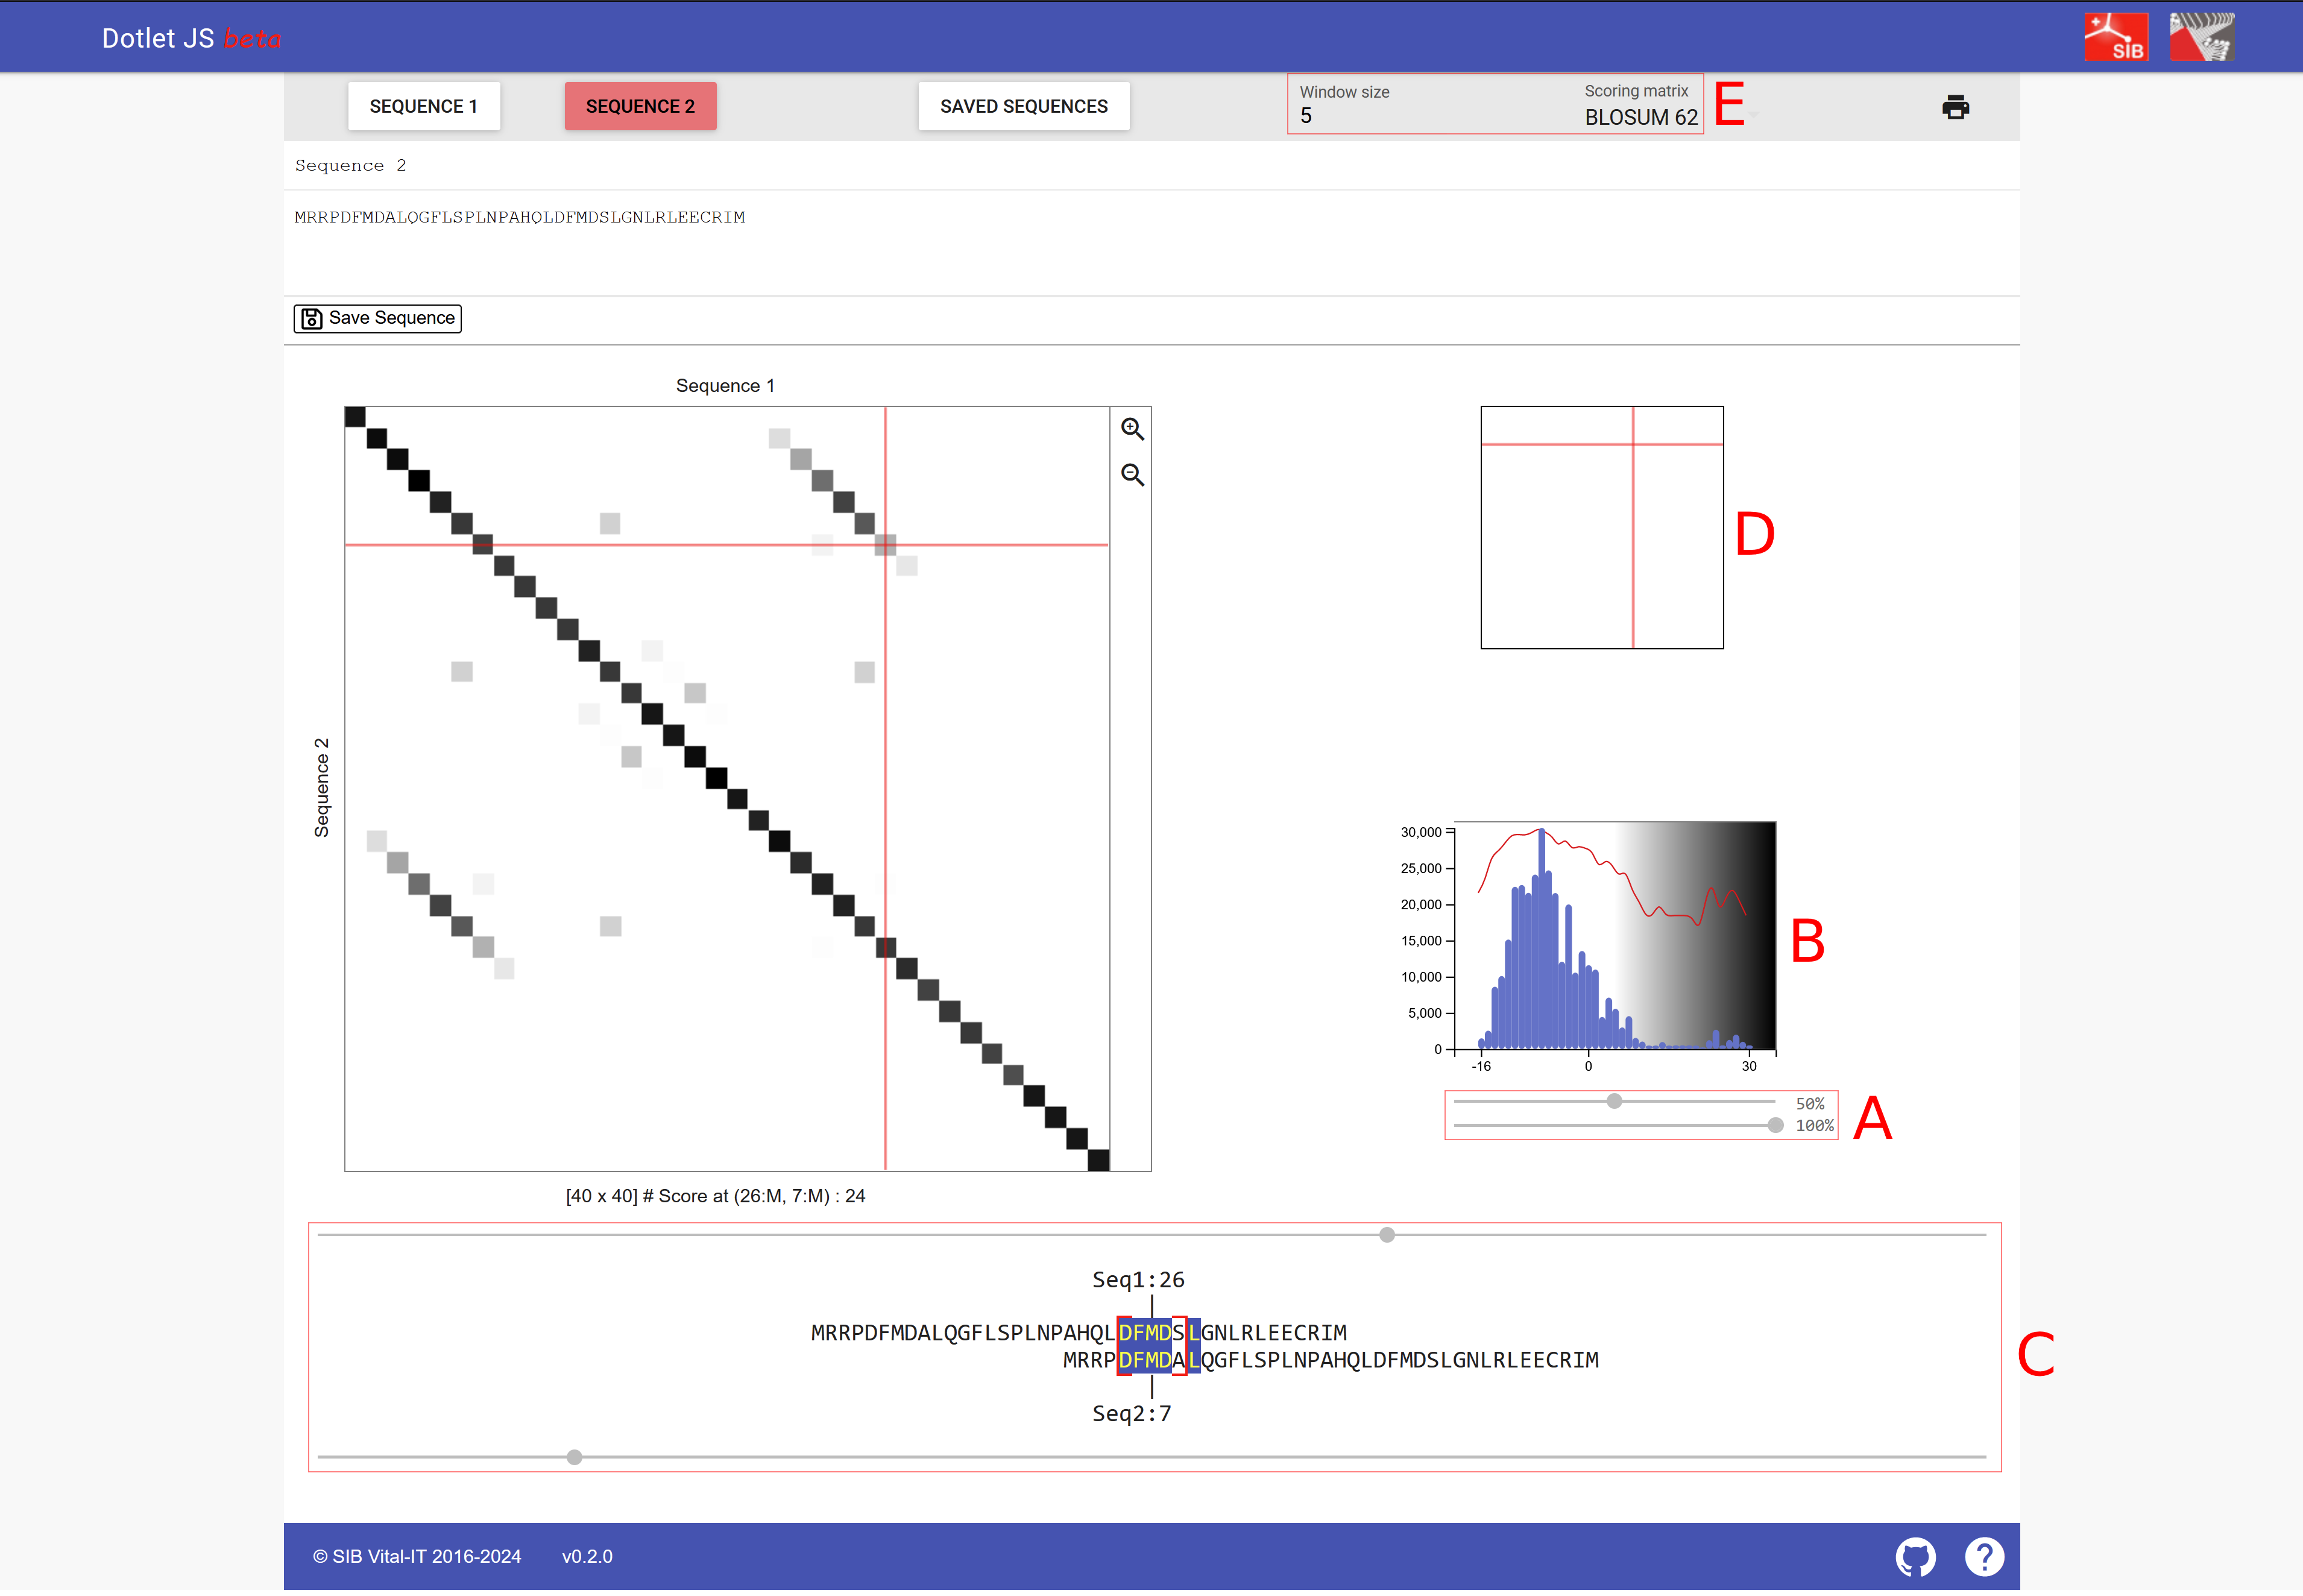
\includegraphics[width=1\linewidth]{files/dot_web-0662600de881673d53ee7891b616612c.png}
\caption[]{A screenshot of \href{https://dotlet.vital-it.ch/}{dotlet} with sequence \texttt{MRRPDFMDALQGFLSPLNPAHQLDFMDSLGNLRLEECRIM}.

\begin{itemize}
\item (A) The two sliders to change the appearence of the plot: The top slider can adjust the sensitivity, moving it to the right, fewer similar regions are shown; moving it to the left, also regions with lower similarity appear.
The bottom slider adjusts the color scheme and is less relevant compared to the top slider.
\item (B) The histogram indicates how many hits with a particular similarity are shown; thus the slider can be adjusted to the right tail of the histogram.
\item (C) The two sliders that can adjust how the two sequences are positioned against each other.
\item (D) Serves a similar function as the two sliders of C but allows for arrow key navigation of the dotplot.
\item (E) Here you can select the window size of sequence comparison and the scoring matrix (window size is explained below and substitution matrices will also be explained below).
\item Credits: \cite{dotlet_2000}.
\end{itemize}}
\label{dotweb}
\end{figure}

\subsection{Pairwise alignment}

Dot plots provide a visual way to compare two sequences, however, they do not provide the similarity between two sequences.
To calculate sequence similarity or sequence identity, we need to perform a \textbf{pairwise sequence alignment}.
In an alignment, the two sequences will be placed above each other and gaps can be introduced to represent insertions or deletions of residues.
We also say that the two sequences will be \textbf{aligned}.
The resulting alignment contains matches, mismatches, and gaps (Figure~\ref{algterm})

\begin{figure}[!htbp]
\centering
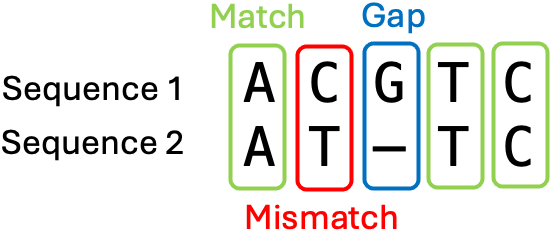
\includegraphics[width=0.5\linewidth]{files/alg_term-f276ccefbf1d202caaf7f23d7464dc58.png}
\caption[]{A small example of two aligned sequences.
Credits: \href{https://creativecommons.org/licenses/by-nc/4.0/}{CC BY-NC 4.0} \cite{own_2_2024}.}
\label{algterm}
\end{figure}

\subsubsection{Alignments of DNA sequences}

Every position in a sequence could potentially have an instertion or a deletion, so there are many possible locations and combinations for gaps and thus many potential alignments.
The final alignment will be the one with the maximum total alignment score.
This score is determined by the scoring parameters that are chosen before the alignment calculation.
An example of DNA sequence scoring paramaters could be that matches score 1 and mismatches -1 and that there is a gap penalty of -1.
The total alignment score is calculated by summing over all columns in the alignment (Figure~\ref{algscore}).

\begin{figure}[!htbp]
\centering
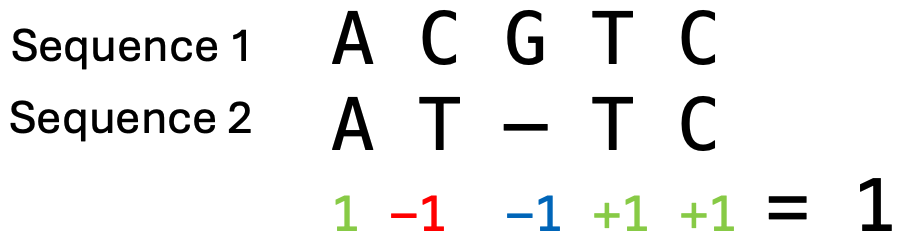
\includegraphics[width=0.6\linewidth]{files/alg_score-2bc8cb8229af1c45cf35062f015e5541.png}
\caption[]{An example calculation of the alignment score, where matches score 1, mismatches -1 and there is a gap penalty of -1.
This results in a total score of 1 for this alignment.
Credits: \href{https://creativecommons.org/licenses/by-nc/4.0/}{CC BY-NC 4.0} \cite{own_2_2024}.}
\label{algscore}
\end{figure}

The choice of the scoring parameters has an impact which alignment will have the maximum score.
To understand the impact of the parameters on the final alignment, fill in table Figure~\ref{algex}.

\begin{figure}[!htbp]
\centering
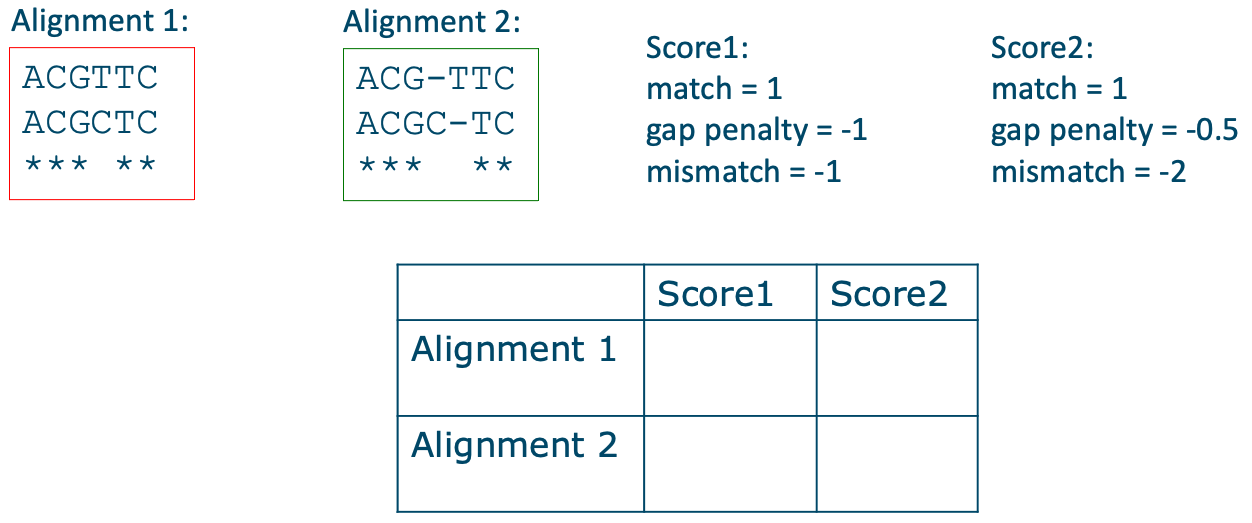
\includegraphics[width=1\linewidth]{files/alg_exercise-44d2e5d97743e3370181c88ae34956bf.png}
\caption[]{\textbf{Assignment}: Fill the table for the two alignments and the two sets of scoring parameters.
Credits: \href{https://creativecommons.org/licenses/by-nc/4.0/}{CC BY-NC 4.0} \cite{own_2_2024}.}
\label{algex}
\end{figure}

\begin{framed}
\textbf{Note 2.1: Affine gap costs}\\
The DNA and protein sequences that we want to align often have varying lengths, which is the result of insertions and deletions during evolution.
Insertion and deletion events can affect one or multiple residues, where one event of length 2 is more likely to happen than two independent events of length 1.
To include this in the scoring scheme, alignment programms use \textbf{affine gap costs} that distinguish between opening a gap and extending a gap.
For example, the default parameters of the pairwise alignment program \href{https://www.ebi.ac.uk/jdispatcher/psa/emboss\_needle}{needle} \cite{EMBL_tools_2022} are:

Gap open (score for the first residue in a gap): -10

Gap extend (score for each additional residue in a gap): -0.5
\end{framed}

\subsubsection{Alignments of protein sequences}

\paragraph{Substitution matrices}\label{chapter2_substitution_matrices}

In chapter~1, we learned that different amino acids have different chemical properties.
When the protein structure and function are conserved, it is more likely that an amino acid gets exchanged by a chemically similar amino acid, compared to a very different one.
When aligning protein sequences, we thus want to penalize the exchange of chemically dissimilar amino acids and reward the exchange of chemically similar amino acids.
To this end, the score of matches and mismatches is generally determined by a \textbf{substitution matrix}, e.g., BLOSUM62 - \textbf{BLOSUM (BLOck SUbstitution Matrix)} (Figure~\ref{blosum62}).
The substitution matrix and the gap parameters then determine the alignment score (Figure~\ref{aa_alg}).

\begin{figure}[!htbp]
\centering
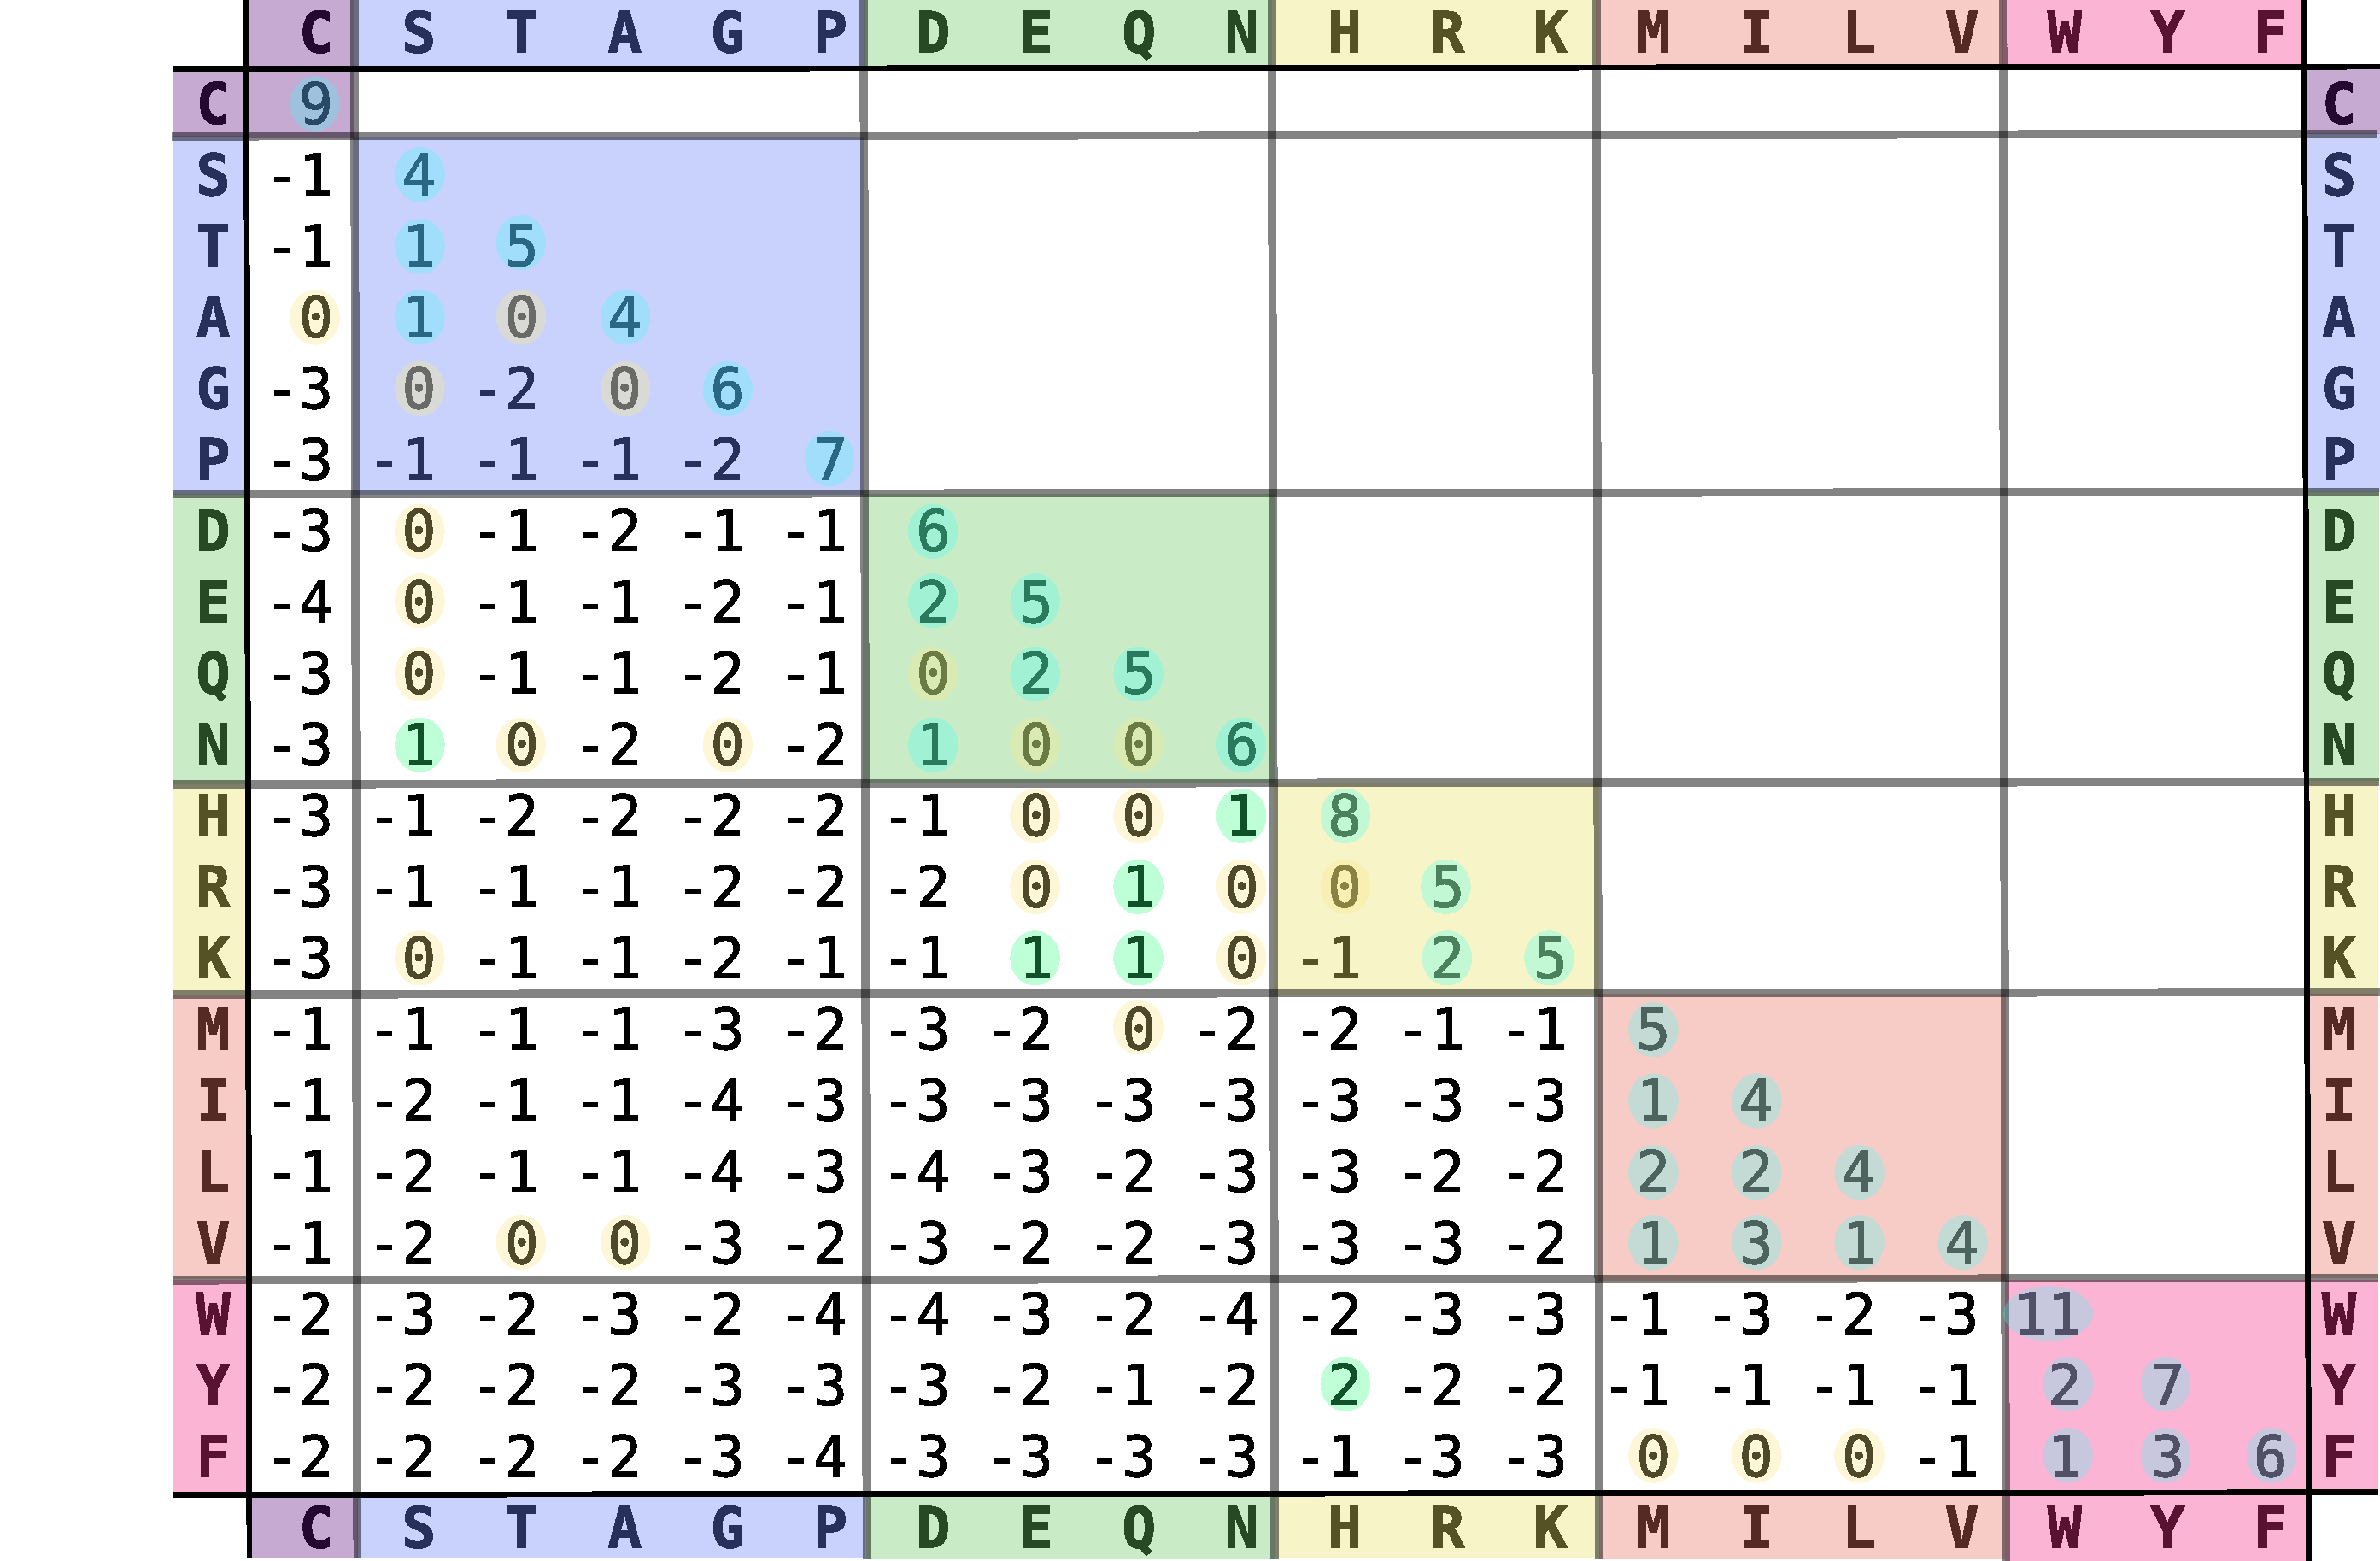
\includegraphics[width=1\linewidth]{files/blosum62-998aa3486f71a507d639852ff7479e95.pdf}
\caption[]{The BLOSUM62 amino acid substitution matrix.
The matrix is ordered and positive values and zero values are highlighted.
Credits: \href{https://creativecommons.org/licenses/by-sa/4.0/}{CC BY-SA 4.0} \cite{blosum62_2022}.}
\label{blosum62}
\end{figure}

\begin{framed}
\textbf{Box 2.1: Assignment}\\
Look at the amino acid properties in the table in chapter~1, choose some amino acids with the same properties and some with different properties.
Then look up these pairs in the BLOSUM62 matrix.
What do you observe?
\end{framed}

\begin{figure}[!htbp]
\centering
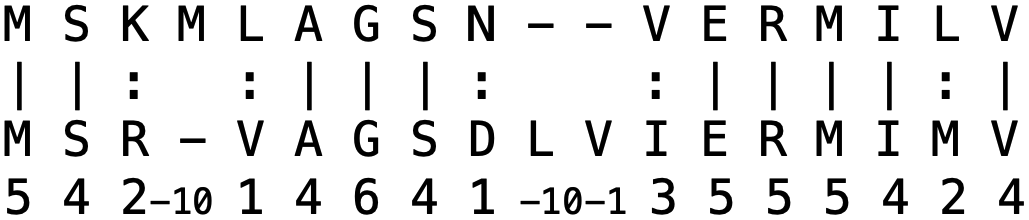
\includegraphics[width=1\linewidth]{files/aa_alg-cf3f1a5e13f7346c86c1b95980331ff4.png}
\caption[]{Example of a pairwise protein alignment.
With the BLOSUM62 scoring matrix, a gap opening score of -10, and a gap extension score of -1, the resulting alignment score is 34.
Credits: \href{https://creativecommons.org/licenses/by-nc/4.0/}{CC BY-NC 4.0} \cite{own_2_2024}.}
\label{aa_alg}
\end{figure}

Note that we motivated the use of amino acid substitution matrices by the chemical properties of amino acids; however, these properties were not directly used when determining these matrices.
Instead, the BLOSUM matrix is determined by aligning conserved regions from Swiss-Prot (chapter~1) and clustering them based on identity.
Then, the substitutions between the different pairs of amino acids within a cluster are counted, which is used to compute the BLOSUM scores.
Thus, these scores reflect directly which amino acids are exchanged more often with each other over evolutionary time and we can observe that this frequency is strongly correlated to their chemical properties.
There are different versions of BLOSUM, for example BLOSUM62 was derived by clustering sequences with an identity of 62\% and it is appropriate for comparing protein sequences having around 62\% identity.
Other available matrices are for example BLOSUM45 and BLOSUM80 (Figure~\ref{submat}).

Another group of matrices that was derived even before BLOSUM is \textbf{PAM (Point Accepted Mutation)}.
The entries in a PAM matrix denote the substitution probabilities of amino acids over a defined unit of evolutionary change.
For example, PAM1 represents one substitution per 100 amino acid residues and is thus appropriate for very closely related sequences.
A commonly used matrix is PAM250, which means that 250 mutations happened over 100 residues; that is, many residues have been affected by more than one mutation.

\begin{figure}[!htbp]
\centering
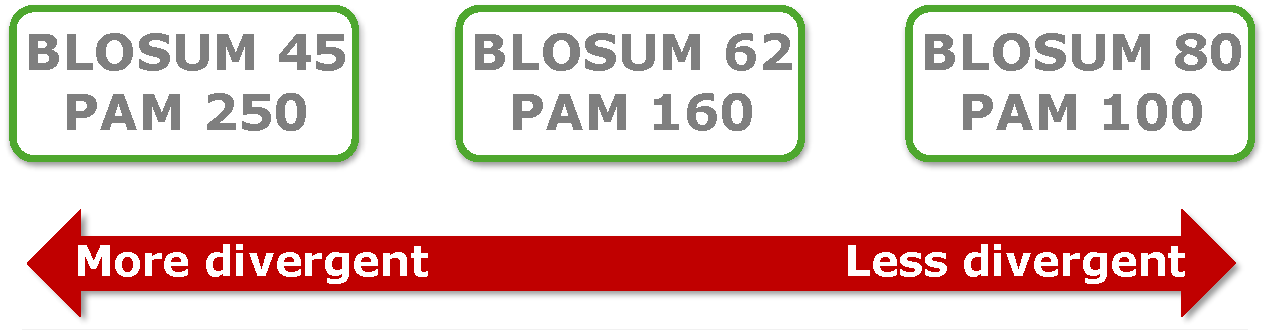
\includegraphics[width=0.8\linewidth]{files/submat-50e39b907c3803a8ca0b3f7fe7f14a07.pdf}
\caption[]{An overview of different available substitution matrices.
Credits: \href{https://creativecommons.org/licenses/by-nc/4.0/}{CC BY-NC 4.0} \cite{own_2_2024}.}
\label{submat}
\end{figure}

\begin{framed}
\textbf{See Also}\\
An introduction into PAM and BLOSUM substitution matrices.
\end{framed}

\paragraph{Protein identity and similarity}

For two protein sequences, we can distinguish two different measures of how much they are alike: identity and similarity, which are defined slightly differently.
The \textbf{protein identity} is given by the number of identical amino acids divided by the alignment length.
The \textbf{protein similarity} is given by the number of similar amino acids \textbf{and} the number of identical amino acids divided by the alignment length.
In the pairwise alignment program \href{https://www.ebi.ac.uk/jdispatcher/psa/emboss\_needle}{needle}, \textbf{identical amino acids} are marked by a pipe symbol/vertical line (|), \textbf{similar amino acids} are marked by a colon (:) and defined by pairs that have a positive score (i.e., \textgreater 0) in the chosen substitution matrix (Figure~\ref{aa_sim}).

\begin{figure}[!htbp]
\centering
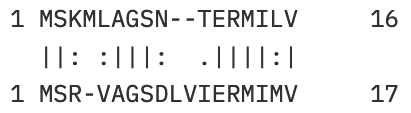
\includegraphics[width=0.6\linewidth]{files/aa_sim-813512ae657cda606e163020688689f4.png}
\caption[]{Example protein alignment. The percent identity is 10 / 18 = 55.6\% and the percent similarity is 14 / 18 = 77.8\%.
Credits: \href{https://creativecommons.org/licenses/by-nc/4.0/}{CC BY-NC 4.0} \cite{own_2_2024}.}
\label{aa_sim}
\end{figure}

Note that the pairwise alignment method does not try to maximize similarity or identity, but they are a result of the chosen parameters.
Especially for distantly related sequences, the parameters can have a big impact on the alignment and thus on the estimated identity and similarity.
In Figure~\ref{alg_gap}, you can find an example of two protein kinases from rice.

\begin{figure}[!htbp]
\centering
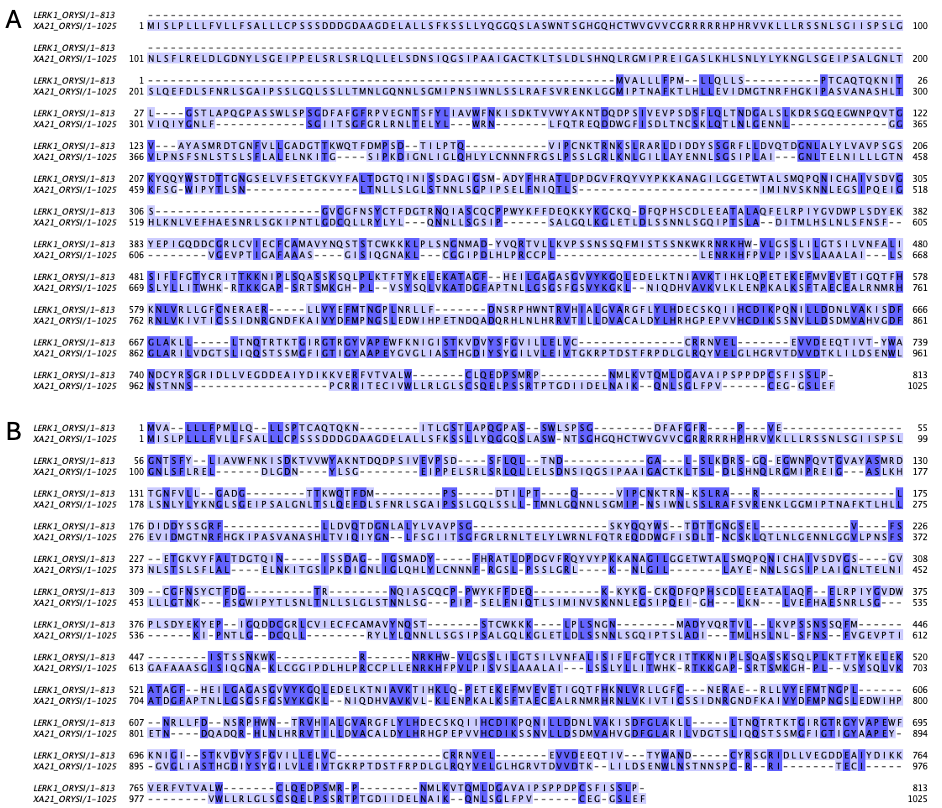
\includegraphics[width=1\linewidth]{files/alg_gap-a25ce3110d8094cc1b4da311bca7e507.png}
\caption[]{Alignments of the same two sequences (LERK1\_ORYSI and XA21\_ORYSI) with different parameters:
A) BLOSUM62 matrix, gap open: -10, gap extend: -0.5. Identity = 210/1191 (17.6\%), Similarity = 345/1191 (29.0\%).
B) BLOSUM62 matrix, gap open: -5, gap extend: -0.5. Identity = 305/1166 (26.2\%), Similarity = 428/1166 (36.7\%).
Credits: \href{https://creativecommons.org/licenses/by-nc/4.0/}{CC BY-NC 4.0} \cite{own_2_2024} made using \href{https://www.ebi.ac.uk/jdispatcher/psa/emboss\_needle}{needle} \cite{EMBL_tools_2022}.}
\label{alg_gap}
\end{figure}

Up until now, we have only considered pairwise alignments, where both sequences are aligned completely, these are called \textbf{global alignments}.

\begin{framed}
\textbf{Note 2.2: Finding the best alignment}\\
There is a huge number of alignments possible for two sequences, since the gaps can be placed in many different ways.
However, to find the \textbf{optimal alignment}, i.e., the one with the highest score, it is not necessary to explore all these possibilities.
Efficient algorithms exist that guarantee to find the optimal alignment.
The Needleman-Wunsch algorithm was the first algorithm and can solve this task in a time that is quadratic to the length of the input sequences.
\end{framed}

\subsubsection{Local alignments}

The previous example shows that some sequences might not be related over their full length.
We have seen in chapter~1 that many proteins are composed of domains.
When comparing two proteins, only some parts that correspond to the domains might be related.
Then, it is more appropriate to perform a \textbf{local alignment}.
Local alignment is also a good tool for identifying functional sites from which sequence patterns and motifs can be derived Figure~\ref{alg_local}.

The aim of a local alignment is to find the best subsequences of both input sequences that result in the maximum alignment score given the alignment parameters.
As for global alignment, efficient algorithms exist to solve this task.
The Smith-Waterman algorithm can also solve this task in a time that is quadratic in the length of the input sequences, just like the Needleman-Wunsch algorithm for global alignments.

\begin{figure}[!htbp]
\centering
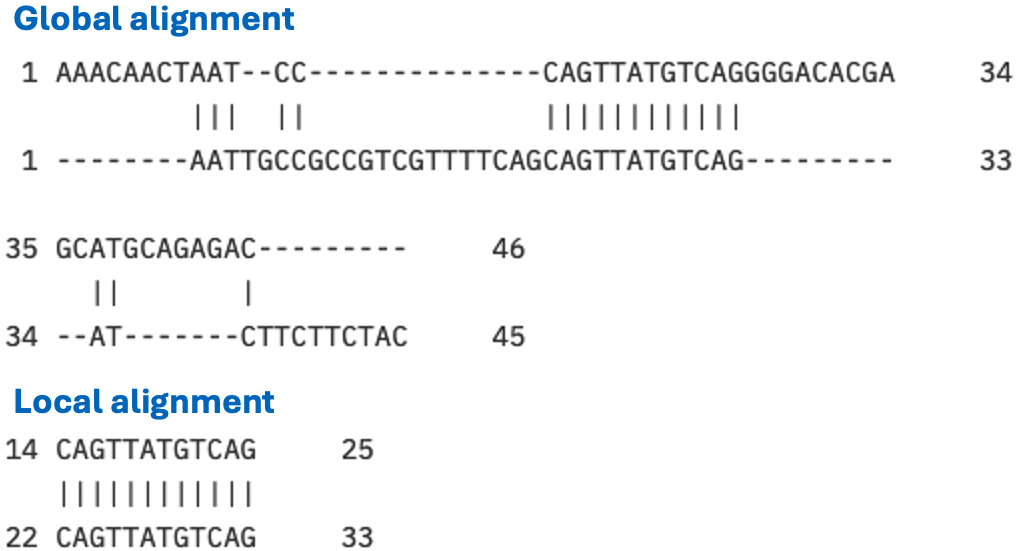
\includegraphics[width=1\linewidth]{files/alg_local-4f60831aa4af06a36d5d4c5a4124517f.png}
\caption[]{Alignments of the same two sequences, once using the global alignment program \href{https://www.ebi.ac.uk/jdispatcher/psa/emboss\_needle}{needle} and once using the local alignment program \href{https://www.ebi.ac.uk/jdispatcher/psa/emboss\_water}{water} \cite{EMBL_tools_2022}.
The same alignment paramters were used: \href{https://rosalind.info/glossary/dnafull/}{DNAfull matrix}, gap open -10, gap extend -0.5.
The global identity is 20/71 (28.2\%) and the local identity is 12/12 (100.0\%).
Credits: \href{https://creativecommons.org/licenses/by-nc/4.0/}{CC BY-NC 4.0} \cite{own_2_2024}.}
\label{alg_local}
\end{figure}

\subsection{Search in sequence databases}\label{chapter2_sequence_search}

In Chapter 1, we learned about different sequence~databases.
We often want to search novel sequences in these databases, for example to learn which other organisms have homologs.
Two sequences that are highly similar, might also share the same function.
This relationship is used for the functional~annotation of sequences, where the search in databases is an important step.

\begin{framed}
\textbf{Note 2.3: Similarity by chance}\\
When all nucleotides occur randomly and at the same frequency, then each sequence of length \texttt{x} is expected to occur with a frequency of 1/4\textsuperscript{x}, e.g., a sequence of length 3 has a frequency of 1/64 and a sequence of length 10 has a frequency of about 1 in a million.
This becomes important since these days, databases are very large, they can contain millions of sequences.
Due to this large amount of data, some similarities might just be observed by chance, especially if our sequence of interest is short.
Thus, statistical methods have been developed to estimate if an observed alignment might have just occured due to chance (see below).
\end{framed}

\subsubsection{Database search vs. pairwise alignment}

Pairwise alignments are also used when searching sequences in sequence databases.
In this task, we have a query sequence and we want to find similar sequences in a database; these similar sequences are called subjects or hits.
Although the algorithms that were discussed in the previous section are relatively fast when two sequences are aligned, it would still take too long overall to perform pairwise sequence alignments of the query with all potential subjects from the database.
We thus need even more efficient algorithms.

\begin{framed}
\textbf{Note 2.4: Heuristic algorithms}\\
The Needleman-Wunsch and the Smith-Waterman algorithm described in the previous section guarantee to find the alignment with the best score for the given sequences and parameters.
In contrast, an \textbf{heuristic algorithm} employs some heuristics, which generally lead to good results and which make the algorithm much faster. However, the method does not guarantee to find the optimal score anymore.
\end{framed}

\subsubsection{BLAST}

Basic Local Alignment Search Tool (\textbf{BLAST}) is a heuristic method to find regions of local similarity between protein or nucleotide sequences.
The program compares nucleotide or protein sequences to sequences in a database and calculates the statistical significance of the matches.
Both the standalone and web version of BLAST are available from the National Center for Biotechnology Information (\href{https://www.ncbi.nlm.nih.gov}{NCBI}).

\paragraph{The algorithm}\label{chapter2_blast_algorithm}

The starting point of BLAST is the set of words that two sequences have in common, where a word is a part of a sequence of a fixed length.
For protein blast, the default word size is 5 and for nucleotide blast it is 11.
To find these common words, first a lookup table of the query words is reconstructed (Figure~\ref{blast_figure}A), where neighborhood words are listed as well.
Neighborhood words are all the words that have a high alignment score with the query word (Figure~\ref{blast_figure}B).
Then, BLAST scans the database for word matches.
For protein blast, two matches within 40 residues must be found such that the BLAST considers the hit as an initial match (Figure~\ref{blast_figure}C).
Note that for nucleotides, initial hits are found in a simpler way:
Only one exact match must be found, i.e., no neighborhood is considered.

After finding initial matches, BLAST extends these matches into local alignments (Figure~\ref{blast_figure}D).
As this extension happens, the alignment score increases or decreases.
When the alignment score drops below a set level, the extension stops.
This prevents the alignment from stretching into areas where there is very little similarity between the query and hit sequences.
If the obtained alignment receives a score above a certain threshold, it will be included in the final BLAST result.
BLAST is thus a heuristic algorithm, but its careful process helps to ensure a reasonable trade-off between run time and accuracy.

\begin{figure}[!htbp]
\centering
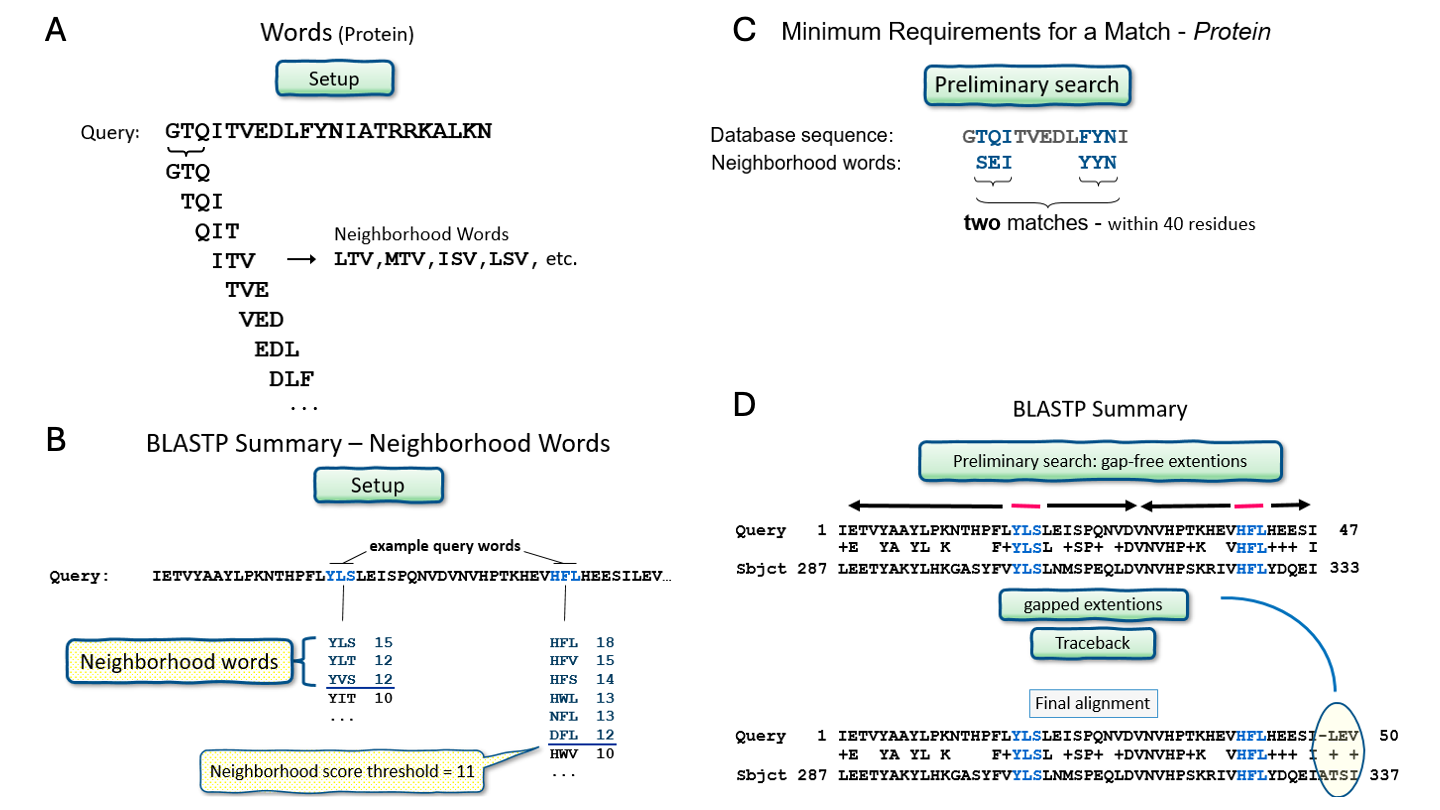
\includegraphics[width=1\linewidth]{files/blast-d0e05e10ecd313dcc8deac97dde44ba2.png}
\caption[]{An overview of the BLAST algorithm.
Credits: \href{https://creativecommons.org/publicdomain/zero/1.0/}{CC0 1.0} \cite{blast_2022}.}
\label{blast_figure}
\end{figure}

\paragraph{BLAST output}

The BLAST output contains vast information on the found hits, their alignments, and taxonomy (Figure~\ref{blast_output}).

\begin{figure}[!htbp]
\centering
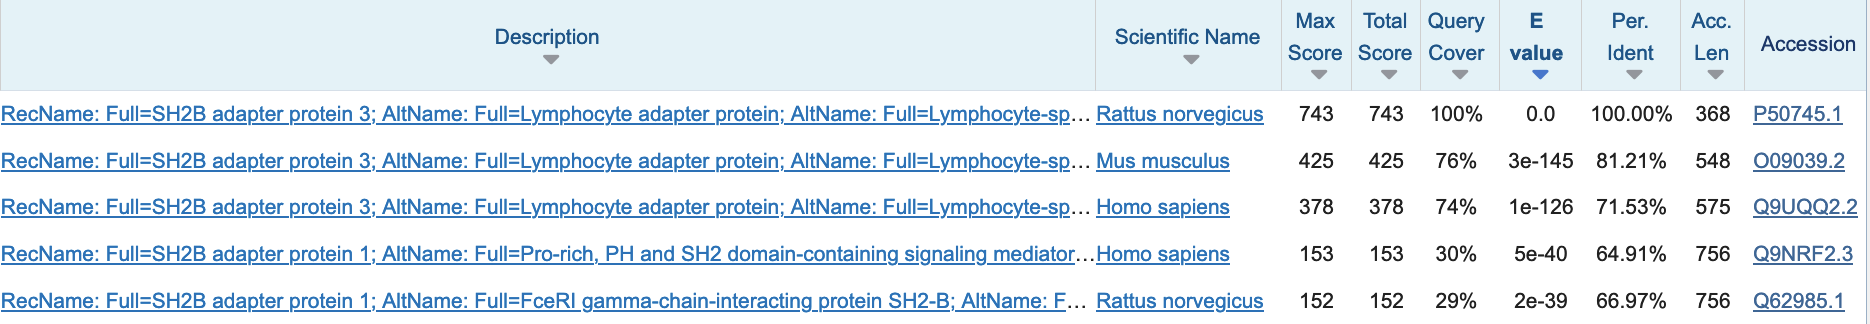
\includegraphics[width=1\linewidth]{files/blast_output-fb4ececca6ae3390731902ad57c4b880.png}
\caption[]{Top 5 blast hits when searching the rat protein P50745 in the Swiss-Prot 2024\_02 release database.
Credits: \cite{blast_2009}}
\label{blast_output}
\end{figure}

\begin{framed}
\textbf{Note 2.5: E-value}\\
An important output statistic is the expectation value (\textbf{e-value}), which is the number of BLAST hits you expect to see by chance in the database, with the observed score or higher.
Note that due to this definition, the e-value depends on the database size.
Since it is more likely to find something by chance in a larger database, the e-value for the same hit would be higher compared to a smaller database.
Thus, to find as many good hits as possible, it makes sense to use the smallest specific database that contains all the sequences you are interested in.
For example, if you are only interested in plants, then restrict your search to only plant sequences.
During the practical you will get to know how to do that in the online BLAST interface.

The BLAST output is sorted by increasing e-value.
This can result in very low numbers and the BLAST output uses the scientific notation to list these, where e.g., 3e-145 means 3*10\textsuperscript{-145}.
Thus, the hits listed in Figure~\ref{blast_output} are likely not random, since their number to be observed by chance is very low.
If the alignment is not by chance, then it might be due to a biological meaningful relationship between the two sequences.
However, it is difficult to define a clear e-value cutoff for biologically meaningful hits.
Commonly used cutoffs are 1e-5 or 1e-10.
\end{framed}

Note that you cannot infer homology by e-value alone, also the coverage and percent identity need to be taken into account.
For example, in Figure~\ref{blast_output}, all hits have very low e-value:
the first hit is to the sequence itself, then there are hits with high identity and high coverage in mouse and human, these might be homologous sequences.
The 4\textsuperscript{th} and 5\textsuperscript{th} hit are only local, since the query cover is {\textasciitilde}30\%, these sequences might only share a homologous domain with the query protein.

\paragraph{BLAST types}

Different types of BLAST exist to search nucleotides or proteins in the respective databases:
\texttt{blastn} searches a nucleotide sequence in a nucleotide database and \texttt{blastp} searches a protein sequence in a protein database.
In addition, the query and/or the database can also be translated in all six reading frames to allow additional kinds of comparisons (Figure~\ref{blast_types}).

% #%[TODO: check that the reading frame translation is clear from chapter 1 or explain more]

Different BLAST types exist for these different kinds of comparisons, where these translations are done automatically (Figure~\ref{blast_types}).

\begin{figure}[!htbp]
\centering
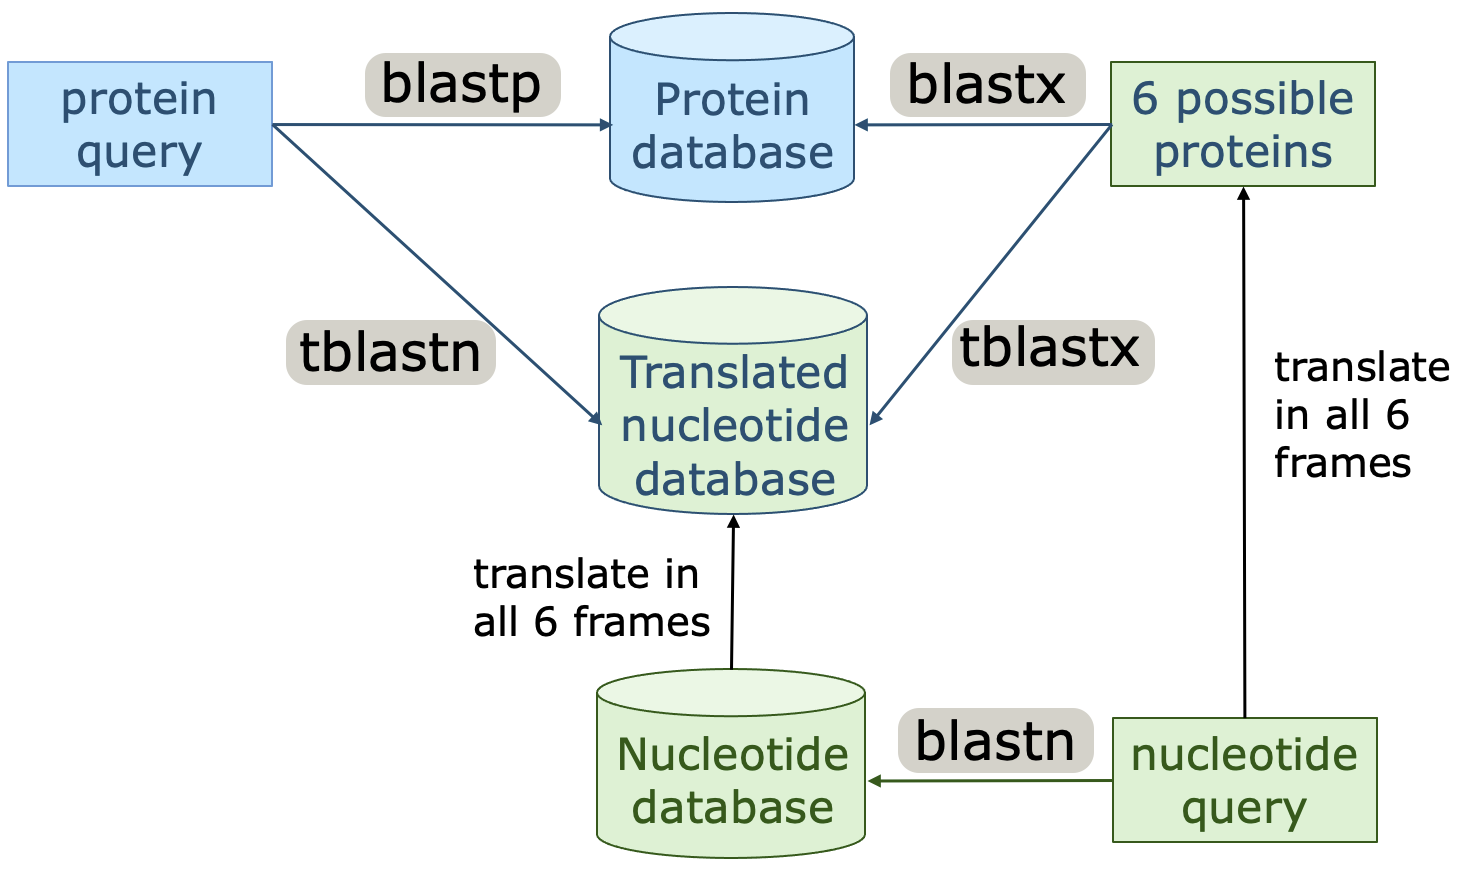
\includegraphics[width=1\linewidth]{files/blast_types-8aed2a3367dbf2bc5c263e0b04d8556e.png}
\caption[]{Different BLAST types to compare different data types. Credits: \href{https://creativecommons.org/licenses/by-nc/4.0/}{CC BY-NC 4.0} \cite{own_2_2024}.}
\label{blast_types}
\end{figure}

% #%[TODO chapter 1: File formats]

\subsection{Multiple sequence alignment}

One straightforward observation from a sequence search is that one query sequence often has multiple similar sequences (Figure~\ref{blast_output}). This can lead to research questions on for example evolution (where do these sequences come from?), function (why are some sequences more similar to each other than to others?), or structure (are all parts of these sequences equally similar/dissimilar?). To compare all of these sequences with each other using a pairwise alignment strategy would quickly lead to a large number of comparisons and would be difficult to interpret. Instead, in cases where we want to compare 3 or more sequences with each other, we turn to \textbf{multiple sequence alignment}.

The objective of performing multiple sequence alignment is to identify matching residues (DNA, RNA, or amino acids) across multiple sequences of potentially differing lengths. Similar to pairwise alignment, the result is called `a multiple sequence alignment'. The resulting multiple sequence alignment can be thought of as a square matrix: rows represent the sequences that we started with, columns represent homologous residues across sequences, and the entries are either residues or gaps (Figure~\ref{msa_concept}).

\begin{figure}[!htbp]
\centering
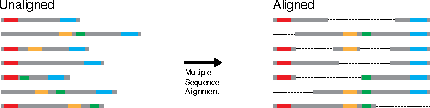
\includegraphics[width=0.8\linewidth]{files/msa-efb05f944d68f64bc1622ab87c647c51.pdf}
\caption[]{Conceptual diagram depicting multiple sequence alignment. Colored dots represent similar sequence elements, in the multiple sequence diagram on the right these elements align in vertical columns. Credits: \href{https://creativecommons.org/licenses/by-nc/4.0/}{CC BY-NC 4.0} \cite{own_2_2024}.}
\label{msa_concept}
\end{figure}

% #% INSERT: SOME SECTION ON RELEVANCE OF MSA

Various algorithms for creating multiple sequence alignments exist. Here we will go over two main concepts that are adopted by many tools: progressive alignment and iterative alignment.

\subsubsection{Progressive alignment}

To avoid having to reconcile many pairwise alignments, progressive alignment takes an iterative approach using a guide tree. The guide tree represents a crude measure of similarity between all sequences that are to be analyzed. Progressive alignment picks the two most similar sequences using the guide tree and initializes the multiple sequence alignment by aligning these two sequences with a global alignment strategy. Subsequently, the guide tree is used to determine the order in which sequences are added to the alignment. One way of thinking about this, is that progressive alignment creates increasingly large `blocks' of sequences, where a block is always treated as a unit (e.g. introducing a gap will happen for all sequences in the block). By iterating through the guide tree, this alignment strategy `progresses' to the final result, hence the name `progressive alignment'.

\begin{framed}
\textbf{Box 2.2: Constructing a guide tree}\\
The guide tree that is used by the progressive alignment strategy is typically created with a clustering algorithm that takes as input all pairwise distances between sequences. Obtaining these pairwise distances can be done through e.g. local alignment scores, but another common approach is to count the number of subsequences of length $K$ (also known as k-mers) that are present in both sequences of a sequence pair. The downside of this k-mer based strategy is that it provides a crude distance measure (and is therefore not very accurate), the benefit is that it is very fast.

In addition, once a multiple sequence alignment has been created with the progressive strategy, it is straightforward to recompute the guide tree based on this first multiple sequence alignment and calculate a second multiple sequence alignment based on this updated guide tree. This recomputing of the guide tree could in theory be repeated infinitely many times, in practice it seems sufficient to only recompute once. The often used multiple sequence alignment program \texttt{mafft} implements recomputing the guide tree in the \texttt{FFT-NS-2} algorithm.
\end{framed}

\subsubsection{Iterative refinement}

One potential downside of the progressive alignment strategy is that some of the intermediate blocks represent sub-optimal alignments. For example, when a gap is introduced during an early stage of the progressive approach, it is never removed from the alignment. Identifying and potentially improving such cases is often referred to as `iterative refinement' and typically happens on a multiple sequence alignment that was created with a progressive strategy.

Iterative refinement takes as input a multiple sequence alignment, a scoring function for the multiple sequence alignment, and a function to rearrange the multiple sequence alignment. It produces a `refined' multiple sequence alignment by rearranging the multiple sequence alignment and only keeps the new multiple sequence alignment if the score has increased. This process is typically repeated untill the score no longer increases (or for a fixed number of iterations).

Since iterative refinement methods typically start with a progressive alignment and improve its score, programs that implement an iterative refinement strategy (e.g., the FFT-NS-i method in \texttt{mafft}) typically perform better, but also need more time, than programs that are based on progressive alignment (e.g., the FFT-NS-2 method in \texttt{mafft} and the Clustal program) \cite{katoh_mafft_2014}.

\begin{framed}
\textbf{Box 2.3: Scoring and rearranging multiple sequence alignments}\\
For iterative refinement, various scoring and rearranging strategies exist. Here we outline a common approach for both: the weighted sum-of-pairs scoring function and the partitioning rearrangement strategy.

\textbf{Weighted sum-of-pairs scoring}: A generalization of the sum-of-pairs method, where the sum-of-pairs method simply calculates and sums all possible pairwise alignment scores. The generalization consists of adding specific weighing factors to each pair, where the weights are determined by the phylogenetic relationship between the sequences.

\textbf{Partitioning rearrangement}: Following a guide tree, the multiple sequence alignment is partitioned into two sub-alignments (or blocks) along each branch of the tree. Each pair of blocks is then realigned, but the resulting alignment is only kept if the score of the realigned blocks has increased.
\end{framed}

\subsection{Motifs}

Having established how to obtain a multiple sequence alignment, we now focus on several interpretations. One thing that all of these interpretations have in common, is that they enable the identification of (and search for) commonly occurring sequence patterns. A frequently used term for a commonly occurring sequence pattern is \textbf{motif}, which we will use from now on. All interpretations of motifs are based on summarizing the \textit{columns} of the multiple sequence alignment, in an attempt to describe commonly occurring residues across all sequences.

\begin{framed}
\textbf{Note 2.5: MSAs VS motifs}\\
Since all motifs are based on multiple sequence alignments, it may seem tempting to use the terms interchangeably. A key distinction is that a motif always represent a commonly occurring pattern, whereas a multiple sequence alignment can also contain regions of low conservation/similarity. In addition, one multiple sequence alignment can contain multiple motifs.
\end{framed}

Arguably the simplest representation of a motif is the \textbf{consensus sequence} (Figure~\ref{motif_concept}B), where every column of the multiple sequence alignment is represented by the most frequently occurring residue (i.e. the majority consensus). The downside of a consensus sequence is that it does not represent any of the variation present in the motif.

An extension of the consensus sequence that can represent some variation in a motif is the \textbf{pattern string} (Figure~\ref{motif_concept}C).
In pattern strings, unambigous positions are represented by single letters and there is a special syntax for representing variation:
Positions in the MSA with more than one character are represented by multiple characters in between square brackets.
A pattern string containing, for example, the pattern \texttt{[AG]} indicates that one position in the motif can be either \texttt{A} or \texttt{G}. As such, pattern strings take inspiration from \href{https://en.wikipedia.org/wiki/Regular\_expression}{regular expressions}. Various types of pattern strings exist, for example \texttt{PROSITE} \textbf{REF} strings used in the Prosite~database contain syntax for representing positions in a motif where the residue is irrelevant (marked by an \texttt{*}). Pattern strings are capable of representing some variation in the motif, but they cannot express how likely the occurence of specific variants is (in the example \texttt{[AG]}, both \texttt{A} and \texttt{G} are equally likely to occur).

To express the likelihood of a specific residue occurring at a specific position, a \textbf{Position Specific Scoring Matrix (\gls{term-pssm})} can be used (Figure~\ref{motif_concept}D).
Every row represents one of the possible characters in the MSA and every column represents a column in the MSA, where numbers indicate the probability of observing a specific character at a specific position.
Hence, every column sums to one.
For example: a DNA PSSM would have four rows, representing the nucleotides \texttt{A}, \texttt{C}, \texttt{G}, or \texttt{T}. The entries represent probabilities of observing a specific residue at a specific position. As a consequence, all columns in a PSSM must sum to one. Since a PSSM contains probabilities, it is relatively straightforward to calculate how well an unknown sequence matches an existing PSSM: assuming independence between positions, one simply multiplies the observation probabilities of the characters in the novel sequence.

Finally, sequence logos are a graphical representation of an alignment (Figure~\ref{motif_concept}E). Every position in the sequence logo represents a position in the MSA, characters are scaled proportional to their probability of being observed at their respective positions (e.g. an unambiguous position has one large character, a position with several options has multiple small characters).

\begin{figure}[!htbp]
\centering
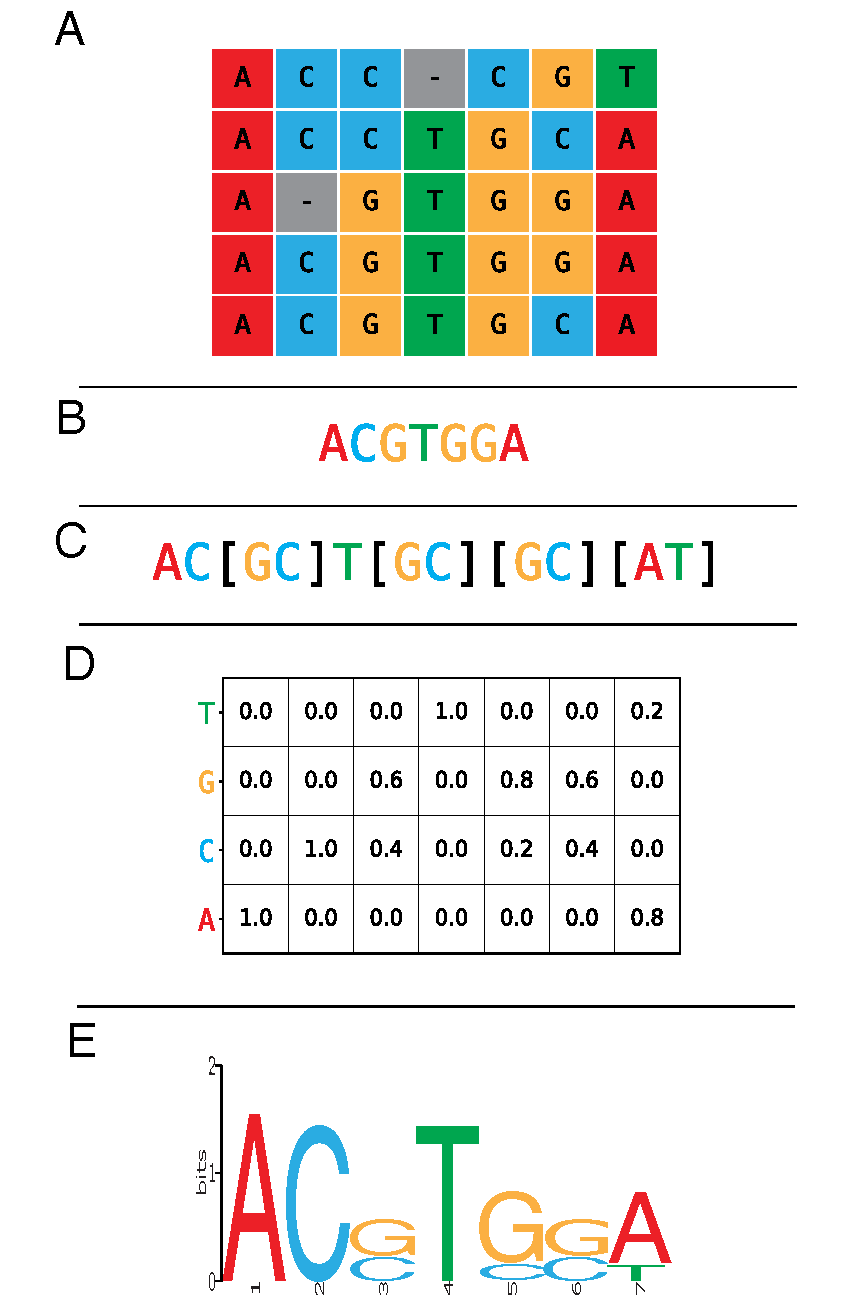
\includegraphics[width=0.6\linewidth]{files/msa-pattern-pssm-log-5b80b466575997384e0c8bd00280fcc2.pdf}
\caption[]{Conceptual diagram depicting various representations of a conserved motif. \textbf{A:} Multiple sequence alignment (MSA) of 5 sequences and 7 positions. \textbf{B:} Consensus sequence. \textbf{C:} Pattern string. \textbf{D:} Position Specific Scoring Matrix (PSSM). \textbf{E:} Sequence logo.
Credits: \href{https://creativecommons.org/licenses/by-nc/4.0/}{CC BY-NC 4.0} \cite{own_2_2024}.}
\label{motif_concept}
\end{figure}

\subsection{Profile hidden Markov models (pHMMs)}

The previous sections on multiple sequence alignments and motifs explained some basics of how collections of similar sequences can be summarized and used. In this section we highlight a powerful approach for using the information in MSAs to perform sequence search and comparison: \textbf{profile hidden Markov models (pHMMs)}. Some of the fundamentals of general hidden Markov models (HMM) have been covered in \href{/chapter1}{Chapter 1}, here we introduce how a few simple adaptations to the general concept of HMMs unlocks a powerful sequence search approach.

The simplest introduction of profile hidden Markov models is to think of them as an extension of a position specific scoring matrix. Like a PSSM, a pHMM contains probabilities of observing certain characters at certain positions in an MSA. However, a pHMM adds the notion that the biological phenomenon of insertion and deletion of sequence elements requires unique distributions of observation probabilities. Following the hidden Markov model formulation: the \textit{hidden states} match/insert/delete all have their own unique \textit{emission probabilities} for the possible characters. In addition, a pHMM includes \textit{transition probabilities} between the  hidden states. A graphical representation of a simple profile HMM can be seen in Figure~\ref{simple_hmm}. Just like in PSSMs, a probabilistic score can be calculated for a novel sequence matching an existing HMM.
Due to the probabilistic nature of HMMs, the length of insertions is in principle unrestricted, whereas particular ranges are defined for PSSMs.
Efficient algorithms for working with pHMMs exist and have been implemented in for example the HMMer suite. The exact details of these algorithms are outside of the scope of this book.

\begin{figure}[!htbp]
\centering
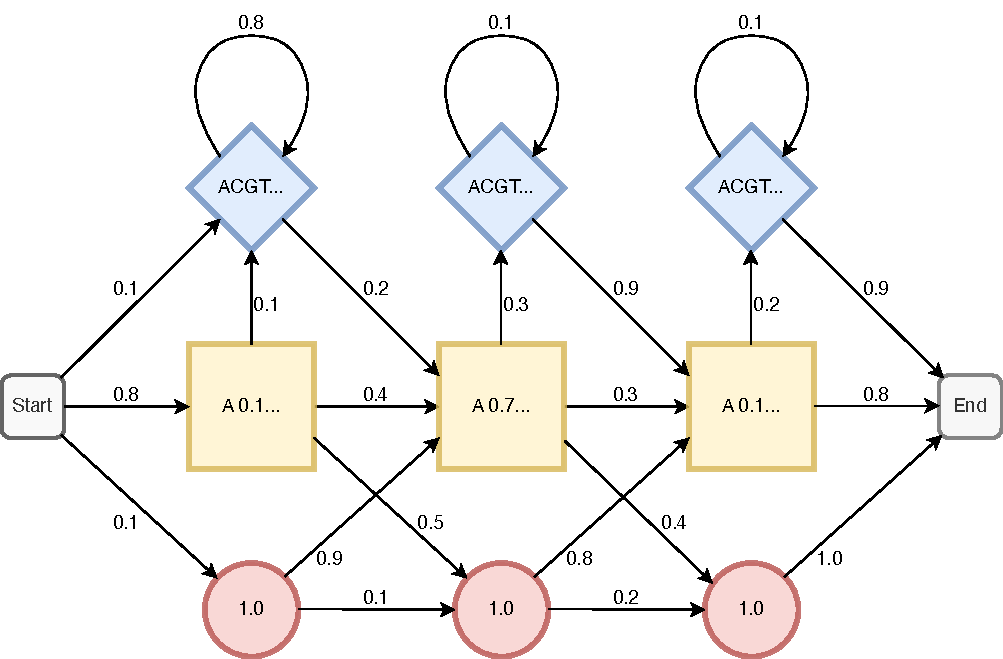
\includegraphics[width=0.6\linewidth]{files/hmm-e0733ae4fec57ce5502f9917dc126281.pdf}
\caption[]{Schematic representation of a simple DNA profile HMM containing all model probabilities. The model consists of three hidden states: match (yellow square), deletion (red circle), and insertion (blue diamond). Emission probabilities are indicated inside the hidden states, transition probabilities between hidden states are indicated next to arrows.
Credits: \href{https://creativecommons.org/licenses/by-nc/4.0/}{CC BY-NC 4.0} \cite{own_2_2024}.}
\label{simple_hmm}
\end{figure}

\begin{framed}
\textbf{Box 2.4: Calculating the probability of a sequence}\\
In principle the information in Figure~\ref{simple_hmm} is enough to calculate the probability of a sequence belonging to this pHMM. For example, the sequence \texttt{GAT} would get a probability of $(0.8 * 0.6) * (0.4 * 0.7) * (0.3 * 0.4) * 0.8 = 0.013$. We arrive at this number by multiplying all relevant transition and emission probabilities. Note that determining the relevant probabilities can be more involved than in this simple example. Efficient algorithms for determining the optimal path through the HMM graph exist, but are outside of the scope of this book. In addition, we do not expect that you can perform these calculation by hand.
\end{framed}

\begin{framed}
\textbf{Sequence search with MSAs}\\
The ability to convert a multiple sequence alignment into a collection of probabilities (e.g. PSSMs or HMMs) makes it possible to calculate the probability of a novel sequence `belonging' to the multiple sequence alignment. This technique generally allows for a more sensitive approach than searching based on pairwise alignments. In practice this often means that matching sequences can be identified over larger evolutionary distances. Tools that implement some version of this approach are \texttt{psiBLAST} (which uses PSSMs) and various \texttt{HMMer} tools (all using pHMMs).
\end{framed}

\begin{framed}
\textbf{Box 2.5: pHMMs in databases}\\
The ability to group biological sequences based on conserved/co-occurring regions and subsequently using this for sequence search is exploited in a wide range of biological sequence databases. Some of these databases have been introduced in \href{/chapter1}{chapter 1}, here we briefly outline a few more details on how HMMs are incorporated into many of these resources by using Pfam as an example. All entries in the PFAM database are represented by profile HMMs. The entries are subdivided into one of six categories: family, domain, repeat, conserved site, coiled coil, or disordered. The main distinction between these six categories is the length of the matching sequences: a `family' PFAM HMM is expected to match across the entire length of a protein sequence, a `conserved site' is typically only a small region in a protein. As such, multiple PFAM HMMs can match a given protein sequence. The combination of matching PFAM HMMs on a given sequence can be used to give a fine-grained description of known elements in a sequence.
\end{framed}

\subsection{PCR primer design}

Many laborary techniques in biomedical applications rely on the polymerase chain reaction (PCR, see box 2.6) for amplifying specific fragments of DNA. Examples include pathogen detection, analyzing genetic variation, targeted mutagenesis, de novo protein synthesis, and studying gene expression patterns. Which DNA fragments are amplified is determined largely by which PCR \textit{primers} are used. To design primers that succesfully amplify the DNA of interest, several computational steps are combined. This section highlight some of these bioinformatic considerations.

\begin{framed}
\textbf{Box 2.6: The polymerase chain reaction (PCR)}\\
Invented in 1983 by Kary B. Mullis, the polymerase chain reaction was first published in 1985 in a study on sickle cell anemia \cite{saiki1985enzymatic}. Ten years after its discovery, PCR's many biomedical applications gained its inventor the 1993 Nobel prize (shared with Michael Smith for his work on site-directed mutagenesis).

As a method for amplifying DNA, PCR relies on the naturally occurring process of DNA replication by the polymerase enzyme to duplicate DNA (See Chapter~1). The reaction uses so-called primers to select which regions of DNA to amplify, and a temperature-cycling scheme to double the number of reaction products in each cycle (Figure~\ref{PCR}). PCR primers are relatively short fragments of single stranded DNA that `prime' the polymerase: they determine where DNA replication should start. Primers always come in pairs: by using a forward and reverse primer at opposing ends and strands of the desired DNA region, it is ensured that two copies of DNA can be made from one original DNA region.

During the reaction, typically three different temperature phases are alternated: (1.) the denaturation phase ({\textasciitilde}95°C) breaks up the double stranded DNA into single stranded DNA, (2.) the annealing phase ({\textasciitilde}55°C) allows the primers to bind to their complementary DNA, forming a small section of double stranded DNA, and (3.) the extension phase ({\textasciitilde}72°C) allows the polymerase enzyme to extend the double stranded section, creating two full double stranded copies of the original material. Repeating this process keeps on doubling the number of copies, which is why it is referred to as a chain reaction.
A crucial discovery in the invention of the PCR reaction for biomedical applications is the use of a polymerase enzyme that can withstand the high temperatures of the denaturation phase. The first thermostable polymerase was extracted from a species of bacteria living in hot springs: \textit{Thermus aquaticus} (hence the name \textit{Taq} polymerase).

\begin{figure}[!htbp]
\centering
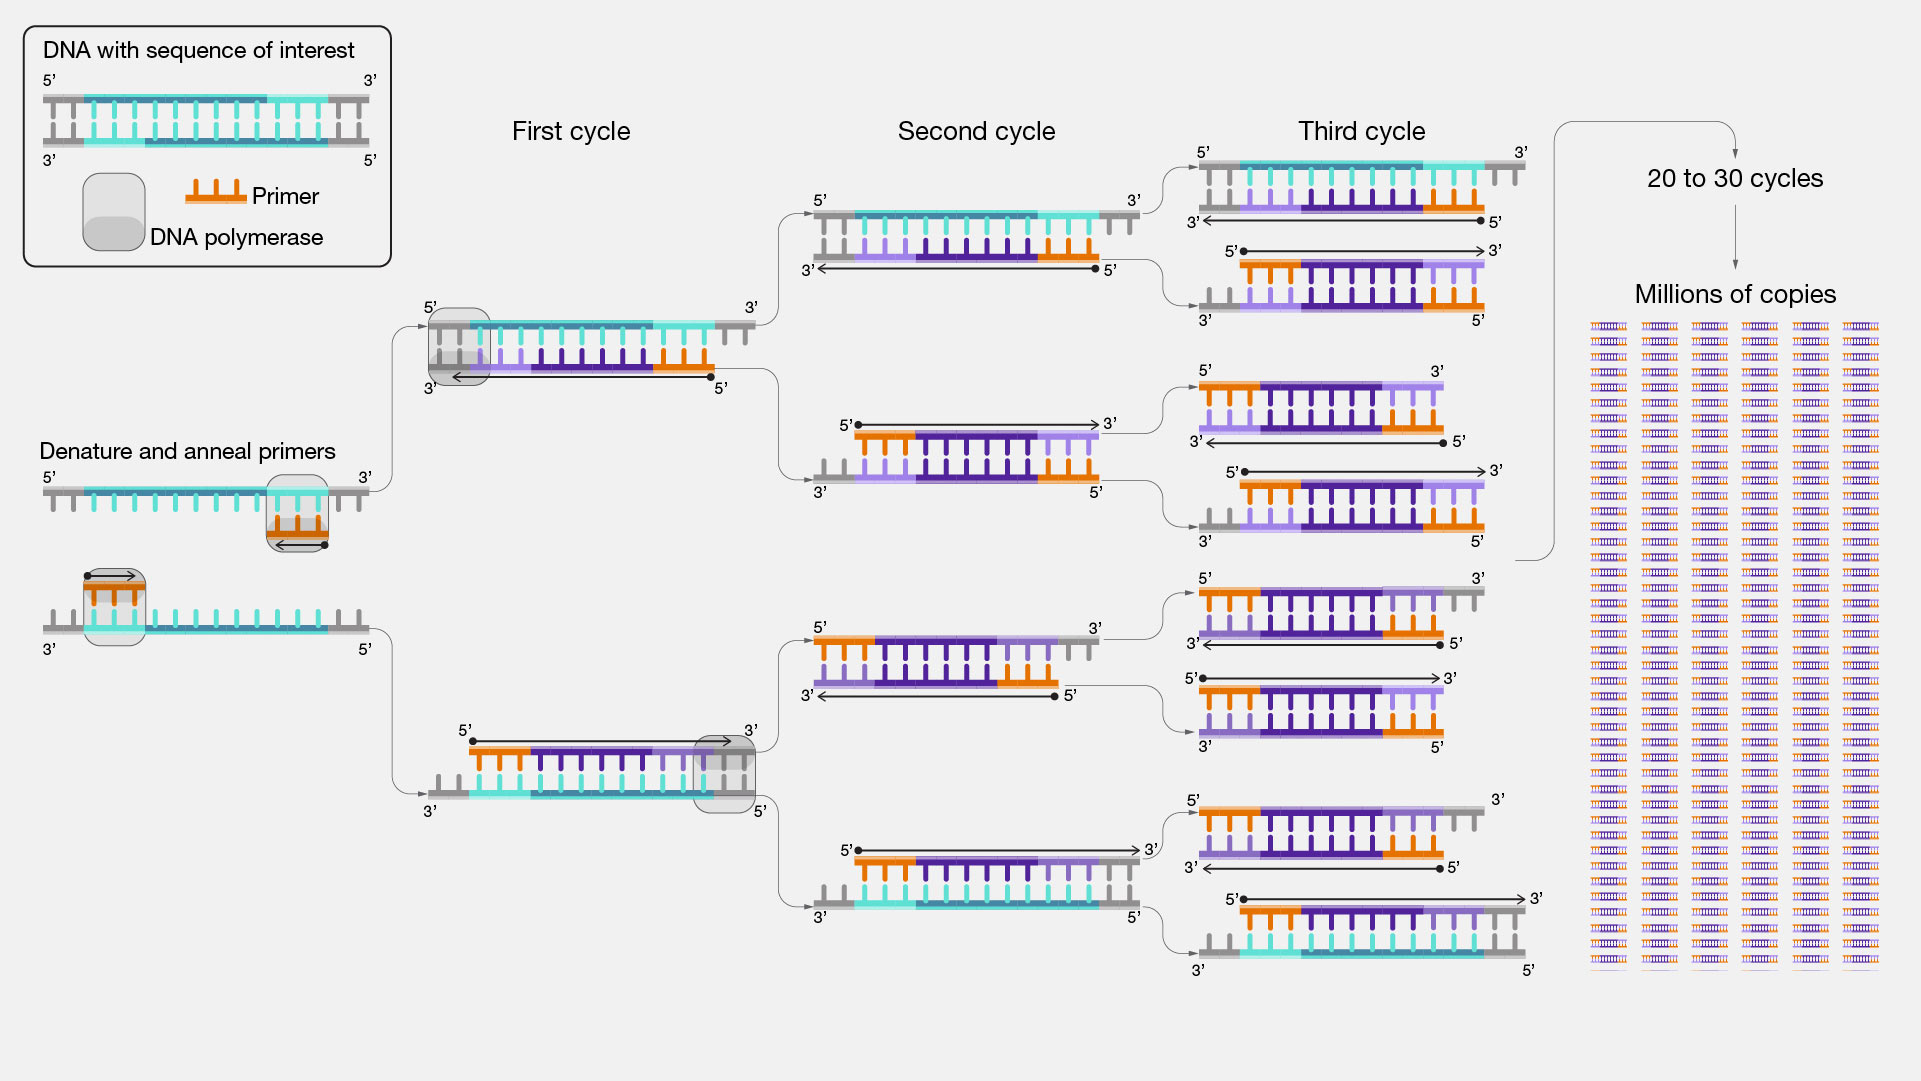
\includegraphics[width=1\linewidth]{files/PCR-2730412a7c2a4e280ab9bfd52d21dbf7.jpg}
\caption[]{The polymerase chain reaction uses primers to select a desired region of DNA, and doubles it's reaction products every cycle.
Credits: \cite{PCR_NHGR}.}
\label{PCR}
\end{figure}
\end{framed}

PCR primers typically have to meet several requirements to result in a successful PCR product: they have to be biochemically feasible (i.e. denature, anneal, and extend at the right temperature), they have to be specific (only amplify the region of interest), they should produce a product of a reasonable size ({\textasciitilde}500-1000 nucleotides, depending on the application), and they should be stable as single stranded DNA. The combination of these requirements typically allows primers of {\textasciitilde}18-30 nucleotides long. To aid in the quick design of potentially successful primers, tools such as Primer-BLAST or Primer3+ automatically check most of the mentioned requirements. For example, Primer-BLAST lets a user upload a sequence of DNA that should be amplified, and can be configured to find primer products of a specific size. In addition, putative off-target amplification (i.e. specificity) is checked using BLAST on a database of choice, and several desired temperatures can be configured.

\begin{framed}
\textbf{Approximating PCR denaturation temperature $T_m$}\\
The temperature at which approximately half of the DNA strands in a solution are in a denatured stated is referred to as the \textit{melting temperature} $T_m$, and is an important parameter in primer design. The exact melting temperature depends on the exact length and nucleotide composition of the DNA fragment, but for short sequences a useful approximation exists. This approximation can come in handy for quick checks and predictions.

For primers shorter than 14 nucleotides, the melting temperature can be approximated with the following formula:

$T_m = 2 * (A + T) + 4 * (G + C)$

Where A, C, G, and T are the number of respective nucleotides in the primer.
\end{framed}


\bigskip
\centerline{\rule{13cm}{0.4pt}}
\bigskip

\subsection{Practical assignments}

This practical contains questions and exercises to help you process the study materials of chapter 2.
There are two supervised practical sessions, one on Wednesday and one on Thursday.
On the first practical day you should aim to get about halfway through this guide.
Thus, you should aim to be finished with Assignment III.
Use the time indication to make sure that you do not get stuck in one assignment.
These practical exercises offer you the best preparation for the project.
Make sure that you develop your practical skills now, in order to apply them during the project.

\textbf{Note, the answers will be published after the practical!}

\begin{framed}
\textbf{\textbf{Project Preparation Exercise}}\\
We continue the project exercise from chapter 1.
Both ARF5 and IAA5 belong to large gene families in \textit{A. thaliana}.
Now, focus on the ARF5 family and explore it by identifying homologs and looking for conserved parts among the family members.
Perform this analysis both within \textit{Arabidopsis thaliana} and outside of this species.
Assess in which plant families members are detected.

Describe the following items in a few bullet points each.
You may include up to two figures or tables.

\begin{enumerate}
\item \textbf{Materials \& Methods} What did you do? Which data, databases and tools did you use, and why did you choose them? What important settings did you select?
\item \textbf{Results} What did you find, what are the main results? Report the relevant data, numbers, tables/figures, and clearly describe your observations.
\item \textbf{Discussion \& Conclusion} Do the results make sense? Are they according to your expectation or do you see something surprising? What do the results mean, how can you interpret them? Do different tools agree or not? What can you conclude? Make sure to describe the expectations and assumptions underlying your interpretation.
\end{enumerate}
\end{framed}

\subsection{Glossary}

\subsection{References}